\chapter{Hardware}
erarbeitet von Leon Kranner und Marcel Wagner \\ \\
\noindent
In diesem Kapitel beschreiben wir die Hardware-Komponenten, die für das Projekt \textbf{Spiegel AI} verwendet wurden. Wir gehen auf die Auswahlkriterien, die Installation und die Konfiguration der Hardware ein.

\section{Komponenten}
Im folgenden Abschritt, werden nun die verwendeten Hardware KOmponenten beschrieben und wofür diese genutzt werden. \\ \\
\noindent
\textbf{Raspberry Pi 3 Model B} \\ \\
Der Raspberry Pi 3 Model B ist das Herzstück des Smartmirrors. Für die Speicherung von Betriebssystem und Daten wird eine 64 GB microSD-Karte verwendet, die ausreichend Platz für alle benötigten Software-Anwendungen bietet. Nachfolgend kann der Raspberry Pi entnommen werden\\ \\
\noindent
\begin{figure}[h]
    \centering
    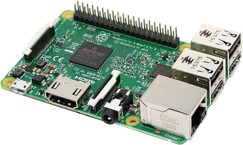
\includegraphics[width=0.3\textwidth]{pictures/raspberry_pi.jpg}
  \captionsetup{justification=centering, labelformat=simple, singlelinecheck=false}
    \caption[Raspberry Pi Model B]{Raspberry Pi Model B\\ Quelle: siehe \cite{raspberry_pi}}
\end{figure} \\ \\
\noindent
\textbf{Logitech Kamera zur Gesichtserkennung} \\ \\
Für die Gesichtserkennung wird eine Logitech Kamera verwendet, die eine hohe Bildqualität und eine zuverlässige Leistung bietet. Diese Kamera ist über USB mit dem Raspberry Pi verbunden und ermöglicht es, Benutzer zu erkennen und auf sie zugeschnittene Informationen anzuzeigen. In der nachfolgenden Abbildung kann die Kamera entnommen werden.\\ \\
\noindent
\begin{figure}[h]
    \centering
    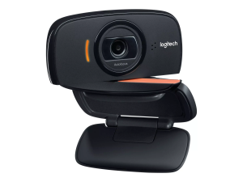
\includegraphics[width=0.3\textwidth]{pictures/logitech_kamera.png}
  \captionsetup{justification=centering, labelformat=simple, singlelinecheck=false}
    \caption[Logitech Kamera]{Logitech Kamera\\ Quelle: siehe \cite{logitech_camera}}
\end{figure} \\ \\
\noindent
\textbf{Monitor} \\ \\
Der Dell Monitor dient als Display für den Smartmirror. Er ist über den integrierten VGA Anschluss mithilfe eines Adapters mit dem Raspberry PI verbunden und ist in das Spiegelgehäuse integriert. Der Monitori wir in der Nachfolgenden Abbildung ersichtlich. \\ \\
\noindent
\begin{figure}[h]
    \centering
    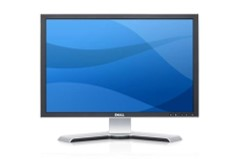
\includegraphics[width=0.3\textwidth]{pictures/dell_monitor.jpg}
  \captionsetup{justification=centering, labelformat=simple, singlelinecheck=false}
    \caption[Dell Monitor]{Dell Monitor\\ Quelle:  siehe \cite{dell_monitor}}
\end{figure} \\ \\
\noindent
\textbf{WLAN Stick} \\ \\
Ein WLAN Stick wird verwendet, um den Raspberry Pi mit dem Internet zu verbinden. Dies ermöglicht die Nutzung von Online-Diensten und die Kommunikation mit anderen Geräten im Netzwerk. Dies ist esentiell um die Funktionsweise des Smart Mirrors zu gewährleisten. \\ \\
\noindent
\textbf{Smartphone} \\ \\
Ein Smartphone dient als mobile Schnittstelle für den Smartmirror. Über eine App können Benutzer Einstellungen vornehmen. Eine genaue beschreibung dieser Schnittstelle erfolgt im Abschnitt (ergänzen). \\ \\
\noindent
\section{Auswahlkriterien}
Die Auswahl der Hardware KOmponenten basierte auf mehrere Kriterien, diese werden nun im folgenden genauer beschrieben:
\begin{itemize}
    \item \textbf{Kompatibilität:} Alle Komponenten mussten kompatibel miteinander und mit der Software-Plattform des Smartmirrors sein.
    \item \textbf{Leistung:} Der Raspberry Pi 3 Model B wurde wegen seiner ausreichenden Rechenleistung und Energieeffizienz gewählt.
    \item \textbf{Bildqualität:} Die Logitech Kamera wurde aufgrund ihrer hohen Auflösung und zuverlässigen Gesichtserkennung ausgewählt.
    \item \textbf{Displayqualität:} Der Dell Monitor bietet eine klare und scharfe Anzeige, was für die visuelle Darstellung der Informationen wichtig ist.
    \item \textbf{Konnektivität:} Der WLAN Stick sorgt für eine stabile Internetverbindung, was für die Nutzung von Online-Diensten unerlässlich ist.
    \item \textbf{Benutzerfreundlichkeit:} Das Smartphone als mobile Schnittstelle erleichtert die Interaktion und die Anpassung der Einstellungen durch den Benutzer.
\end{itemize}
\section{Installation}
In diesem Abschnitt wird nun die einzelnen schritte beachtet, welche bei der installierung der unterschiedlichen Hardware Komponennten vorgegangen sind. \\ \\
\noindent
\textbf{Raspberry Pi 3 Model B}
\begin{itemize}
    \item Die microSD-Karte wurde formatiert und das Betriebssystem wurde darauf installiert.
    \item Der Raspberry Pi wurde in das Gehäuse eingebaut und mit dem Monitor über den VGA auf HDMI Adapter verbunden.
    \item Die Stromversorgung wurde angeschlossen und der Raspberry Pi wurde gestartet.
\end{itemize}
\vspace{0.5cm}
\noindent\textbf{Logitech Kamera}
\begin{itemize}
    \item Die Kamera wurde über USB mit dem Raspberry Pi verbunden.
\end{itemize}
\vspace{0.5cm}
\noindent\textbf{Monitor}
\begin{itemize}
    \item Der Monitor wurde in das Spiegelgehäuse integriert und mit dem Raspberry Pi verbunden.
\end{itemize}
\vspace{0.5cm}
\noindent\textbf{WLAN Stick}
\begin{itemize}
    \item Der WLAN Stick wurde in einen freien USB-Port des Raspberry Pi eingesteckt.
\end{itemize}
\vspace{0.5cm}
\noindent\textbf{Smartphone}
\begin{itemize}
    \item Eine spezielle App wurde auf dem Smartphone installiert, um die Kommunikation mit dem Smartmirror zu ermöglichen.
    \item Das Smartphone wurde mit dem WLAN des Raspberry Pi verbunden
\end{itemize}

\section{Konfiguration}
Ich folgenden Abschnitt wird nun beschrieben wie die unterschiedlichen Hardware Komponenten Konfiguriert wurden. \\ \\
\noindent
\textbf{Logitech Kamera:}
Die Gesichtserkennungssoftware wurde installiert und entsprechend kalibriert. Desweiteren wurden die Kameraeinstellungen angepasst, um eine optimale Erkennungsrate zu gewährleisten. \\ \\
\noindent
\textbf{Monitor (Dell):}
Die Bildschirmeinstellungen wurden so konfiguriert, dass der Monitor im Energiesparmodus bleibt, wenn der Smartmirror nicht verwendet wird. Des weiteren wurde die Anzeigesoftware für den Smartmirror installiert und konfiguriert. \\ \\
\noindent
\textbf{Smartphone:}
Die App auf dem Smartphone wurde installiert.

\subsection{Konfiguration des Raspberry Pi}
\textit{Erarbeitet von David Vollmer.} \\ \\
Die Konfiguration des Raspberry Pi ist im Vergleich zu der der anderen Hardware recht umfangreich. Da ich zuvor noch nie mit einem Raspberry Pi gearbeitet habe, sind in diesem Prozess einige Probleme aufgetreten. Das erste Problem kam schon beim Versuch, ein Betriebssystem zu installieren. Ich habe zwar schon oft Windows und Linux-Distributionen installiert, bis jetzt jedoch nur auf Laptops und Desktop-PCs. Deswegen ging ich davon aus, dass Raspberry Pi OS, welches ein auf Debian basiertes Betriebssystem ist, via USB eingerichtet wird.\cite{raspi_os} Es stellte sich heraus, dass sowohl die Speicherung als auch die Installation mit Hilfe einer microSD Speicherkarte ausgeführt wird. Nachdem das Betriebssystem aufgesetzt wurde, kam eine weitere Schwierigkeit hinzu. Die Verbindung zum Internet war zwar durch ein Ethernet-Kabel möglich, kabellos funktionierte sie aber nicht. Laut Spezifikation ist der Raspberry Pi 3 Model B mit einem drahtlosen Kommunikationschip, inklusive WLAN, ausgestattet.\cite{raspberry_pi} Der Versuch, dieses Problem durch Updates der Netzwerktreiber zu beheben scheiterte. Daraufhin gingen wir von einem Hardwaredefekt aus. Da der Spiegel AI ohne Internetzugriff nicht funktionieren kann und das Anschließen eines Ethernet-Kabels im Betrieb unpraktikabel ist, entschieden wir uns dazu, die drahtlose Verbindung mithilfe eines USB WLAN-Sticks herzustellen. Um diesen zum Laufen zu bekommen, mussten wir Treiber suchen, welche auf dem Betriebssystem funktionieren. Bei den ersten zwei Treibern, die ich versuchte zu installieren, gab es Dependecy-Errors. Das bedeutet, dass zur Installation benötigte Pakete fehlten. In beiden Fällen traten diese Fehler nach über 20 Minuten des Installationsprozesses auf. Der dritte Versuch eines Treiber-Downloads war nach etwa 40 Minuten Wartezeit erfolgreich und der Raspberry Pi konnte erfolgreich auf das Internet zugreifen. Um nun auf die Software des Spiegel AI zuzugreifen, klonte ich das git-Repository des Projekts. Im nächsten Schritt war es nötig, Bibliotheken für die verwendeten Python-Programme herunterzuladen. Diese Libraries waren unter anderem benötigt für den Websocket und für die Gesichtserkennung mit OpenCV. Hierbei war meine Erfahrung mit Linux-Distributionen, unter anderem auch Debian, sehr hilfreich, da ich mit dem Suchen und Installieren korrekter Pakete vertraut bin. Außerdem fiel mir die Navigation im Terminal und das Nutzen gängiger Shell-Befehle sehr leicht, was die Arbeitszeit in diesem Schritt vergleichsweise kurz hielt. Ein zukünftiger Schritt, welcher für die Verwendung des Spiegel AI nützlich sein kann, ist das automatische Starten der nötigen Applikationen. Hierbei müssen der Websocket-Server, der HTTP-Server und die Gesichtserkennung im Hintergrund und die Spiegelanzeige im Vordergrund gestartet werden. Erzielt werden kann dies, indem man Service-Dateien beschreibt, welche beispielsweise BASH-Skripte ausführen lassen. Nachdem die Services eingeschaltet sind, führen sie die Programme nach dem Hochfahren des Systems aus. Der Grund, weshalb dies noch nicht konfiguriert ist, liegt an der Volatilität des Gesichtserkennungsprogramm. Dieses tendiert nämlich dazu, abzustürzen. Das bedeutet, dass oft Intervention mit Eingabeperipherie nötig ist, was den Nutzen des automatischen Starts verringert. Sobald dieses Problem behoben ist, führt diese Änderung jedoch zu einer deutlichen Verbesserung des Nutzererlebnisses, da der Spiegel AI dann ohne Eingabe-Hardware vollständig nutzbar ist.